\subsection{邻域}

定义 4. 设 X 是拓扑空间，A 是 X 的任一子集。A 的邻域是 X 中包含一个含 A 的开集的任一子集。由单独一点组成的子集 \(\{x\}\) 的邻域也称为点 x 的邻域。

显然，X 的子集 A 的每个邻域也是每个子集 \(B \subset A\) 的邻域；特别地，它是 A 的每个点的邻域。反之，设 A 是集合 B 的每一点的邻域，并设 U 是含于 A 的诸开集之并；则 \(U \subset A\)，且由于 B 的每一点都属于某个含于 A 的开集，我们有 \(B \subset U\)；而由 \((\mathrm{O}_{\mathrm{I}})\)，U 是开集，故 A 是 B 的邻域。特别地：

命题 1. 集合是它的每个点的邻域，当且仅当它是开集。

“邻域”一词的日常含义使得涉及邻域这一数学概念的许多性质表现为直观性质的数学表达；因此选用这个术语的好处是使语言更富有表现力。为此，在某些陈述中还可以使用“充分接近”与“要多接近有多接近”这样的表述。例如，命题 1 可以陈述成如下形式：集合 A 是开集，当且仅当对每个 \(x \in A\)，所有充分接近 x 的点都属于 A。更一般地，如果一个性质在点 x 的某个邻域的所有点处都成立，我们就说该性质在充分接近点 x 的所有点处成立。

用 \(\mathfrak{B}(x)\) 表示 \(x\) 的所有邻域所成之集。诸集合 \(\mathfrak{B}(x)\) 具有下列性质：

\((\mathbf{V}_{\mathbf{I}})\) \(\mathbf{X}\) 中包含一个属于 \(\mathfrak{B}(x)\) 的集合的每个子集，本身属于 \(\mathfrak{B}(x)\)。

\((V_{II})\) \(\mathfrak{B}(x)\) 中集合的每个有限交属于 \(\mathfrak{B}(x)\)。

\((V_{\mathrm{III}})\) 元素 \(x\) 属于 \(\mathfrak{B}(x)\) 的每个集合。

事实上，这三条性质是定义 4 与公理 (O \(_{II}\) ) 的直接推论。

\((V_{IV})\) 如果 V 属于 \(\mathfrak{B}(x)\)，则存在一个属于 \(\mathfrak{B}(x)\) 的集合 W，使得对每个 \(y \in W\)，V 属于 \(\mathfrak{B}(y)\)。

由命题 1，可取 W 为包含 x 且含于 V 的任一开集。

这条性质可以表述为：x 的一个邻域也是充分接近 x 的所有点的邻域。

诸集合 \(\mathfrak{B}(x)\) 的这四条性质是特征性质。确切地说，我们有：

命题 2. 如果对每个元素 \(x\)（属于一个集合 \(\mathbf{X}\)）都对应了一个子集族 \(\mathfrak{B}(x)\)，它由 \(\mathbf{X}\) 的子集组成，且使得性质 \((\mathbf{V}_{\mathbf{I}}), (\mathbf{V}_{\mathbf{II}}), (\mathbf{V}_{\mathbf{III}})\) 与 \((\mathbf{V}_{\mathbf{IV}})\) 成立，则在 \(\mathbf{X}\) 上存在唯一的拓扑结构，使得对每个 \(x \in \mathbf{X}\)，\(\mathfrak{B}(x)\) 是该拓扑中 \(x\) 的邻域全体所成之集。

由命题 1，如果 X 上存在满足这些条件的拓扑，则该拓扑的开集全体必是集合 \(\mathfrak{D}\)——X 的这样的子集 A 所成之集：对每个 \(x \in \mathbf{A}\) 有 \(\mathbf{A} \in \mathfrak{B}(x)\)；由此可得该拓扑（若存在）的唯一性。

集合 \(\mathfrak{D}\) 当然满足公理 \((\mathrm{O_I})\) 与 \((\mathrm{O_{II}})\)：对 \((\mathrm{O_I})\) 而言，这由 \((\mathrm{V_I})\) 立即得出；对 \((\mathrm{O_{II}})\) 而言，则由 \((\mathrm{V_{II}})\) 得出。尚须证明，在由 \(\mathfrak{D}\) 定义的拓扑中，\(\mathfrak{B}(x)\) 是 \(x\) 的邻域全体（对每个 \(x \in \mathbf{X}\)）。由 \((\mathbf{V}_{\mathbf{I}})\)，\(x\) 的每个邻域都属于 \(\mathfrak{B}(x)\)。反之，设 \(\mathbf{V}\) 是属于 \(\mathfrak{B}(x)\) 的一个集合，并设 \(\mathbf{U}\) 是点 \(y \in \mathbf{X}\) 全体所成之集，其中 \(\mathbf{V} \in \mathfrak{B}(y)\)；如果能证明 \(x \in \mathbf{U}\)、\(\mathbf{U} \subset \mathbf{V}\) 与 \(\mathbf{U} \in \mathfrak{D}\)，则证明即告完成。我们有 \(x \in \mathbf{U}\)，因为 \(\mathbf{V} \in \mathfrak{B}(x)\)；又有 \(\mathbf{U} \subset \mathbf{V}\)，因为每个点 \(y \in \mathbf{U}\) 都属于 \(\mathbf{V}\)，这由 \((\mathbf{V}_{\mathbf{III}})\) 与假设 \(\mathbf{V} \in \mathfrak{B}(y)\) 得出。尚须证明 \(\mathbf{U} \in \mathfrak{D}\)，即 \(\mathbf{U} \in \mathfrak{B}(y)\) 对每个 \(y \in \mathbf{U}\) 成立；于是（图 1）若 \(y \in \mathbf{U}\)，则由 \((\mathbf{V}_{\mathbf{IV}})\)，存在一个集合 \(\mathbf{W}\)，使得对每个 \(z \in \mathbf{W}\) 有 \(\mathbf{V} \in \mathfrak{B}(z)\)；由于 \(\mathbf{V} \in \mathfrak{B}(z)\) 意味着 \(z \in \mathbf{U}\)，故得 \(\mathbf{W} \subset \mathbf{U}\)，从而由 \((\mathbf{V}_{\mathbf{I}})\) 得 \(\mathbf{U} \in \mathfrak{B}(y)\)。证毕。

\pandocbounded{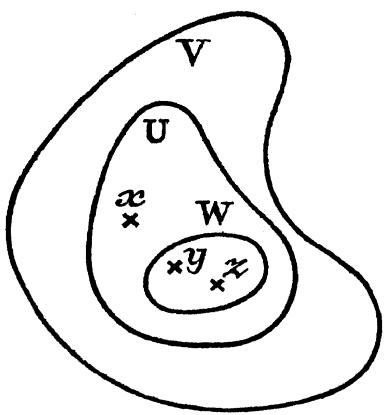
\includegraphics[keepaspectratio]{images/part001_56c83e78.jpg}}\\
图 1.

命题 2 表明，X 上的拓扑可以借助 X 的点的邻域所成之集 \(\mathfrak{B}(x)\) 来定义，只须它们满足公理 \((\mathrm{V}_{\mathrm{I}})\)、\((\mathrm{V}_{\mathrm{II}})\)、\((\mathrm{V}_{\mathrm{III}})\) 与 \((\mathrm{V}_{\mathrm{IV}})\)。

例。我们可以在有理数集合 \(\mathbf{Q}\) 上定义一个拓扑，其开集取为所有有界开区间的并；这些子集所成之集当然满足 \((\mathrm{O}_{\mathbf{I}})\)，而要看出它满足 \((\mathrm{O}_{\mathbf{II}})\)，只须注意：若两个开区间 \(]a, b[\) 与 \(]c, d[\) 的交不空，则它是区间 \(]\alpha, \beta[\)，其中 \(\alpha = \sup (a, c)\) 与 \(\beta = \inf (b, d)\)。对每个 \(x \in \mathbf{Q}\)，把邻域所成之集 \(\mathfrak{B}(x)\)（即 \(x\) 的邻域全体）定义为包含某个含 \(x\) 的开区间的子集全体，就得到同一个拓扑。把该拓扑赋予 \(\mathbf{Q}\) 所得到的拓扑空间称为有理直线（参见第四章，§ 1，第 2 目）。注意，在此空间中每个开区间都是开集。* 我们可以用同样的方式在实数集合 \(\mathbf{R}\) 上定义拓扑；赋有该拓扑的 \(\mathbf{R}\) 称为实直线（参见 § 2，习题 5 及第四章，§ 1，第 3 目）。*

